\documentclass{cubeamer}

\usepackage{trimclip}
\usepackage{wrapfig}
\usepackage{graphicx}
\usepackage{caption}
\usepackage{subcaption}
\usepackage{tikz}
\usetikzlibrary{positioning}
\usetikzlibrary{arrows.meta}
\usetikzlibrary{arrows,shapes,quotes}
\usepackage{amsmath,amsfonts}

\title{Intuitionistic Proofs from Classical Provers}
\subtitle{A new approach to program synthesis}
\author[Alexander Pluska]{Alexander Pluska}
\date{\today} % or whatever the date you are presenting in is
\institute[TU Wien]{TU Wien}
% \copyrightnotice{Published by the American Institute of Aeronautics and Astronautics, Inc., with permission}

\begin{document}
	
	\maketitle
	
	
	\begin{frame}{Motivation}		
		\begin{figure}[!tbp]
			\begin{subfigure}[t]{0.48\textwidth}
				\noindent We have a prover...
				\begin{center}
					
\includegraphics[width=0.8\textwidth]{Vampire.png}
					\includegraphics[width=\textwidth]{CASC.png}
					\caption{CASC-28 Results}
				\end{center}
				\vfill
			\end{subfigure}
			\begin{subfigure}[t]{0.48\textwidth}
				\hfill
			\end{subfigure}
		\end{figure}
	\end{frame}
	
	\begin{frame}{Motivation}		
			\begin{figure}[!tbp]
				\begin{subfigure}[t]{0.48\textwidth}
					\noindent We have a prover...
					
					\begin{center}
						
\includegraphics[width=0.8\textwidth]{Vampire.png}
						\includegraphics[width=\textwidth]{CASC.png}
						\caption{CASC-28 Results}
					\end{center}
					\vfill
				\end{subfigure}
				\begin{subfigure}[t]{0.48\textwidth}
					\hfill...and proofs are programs.
					\begin{center}
						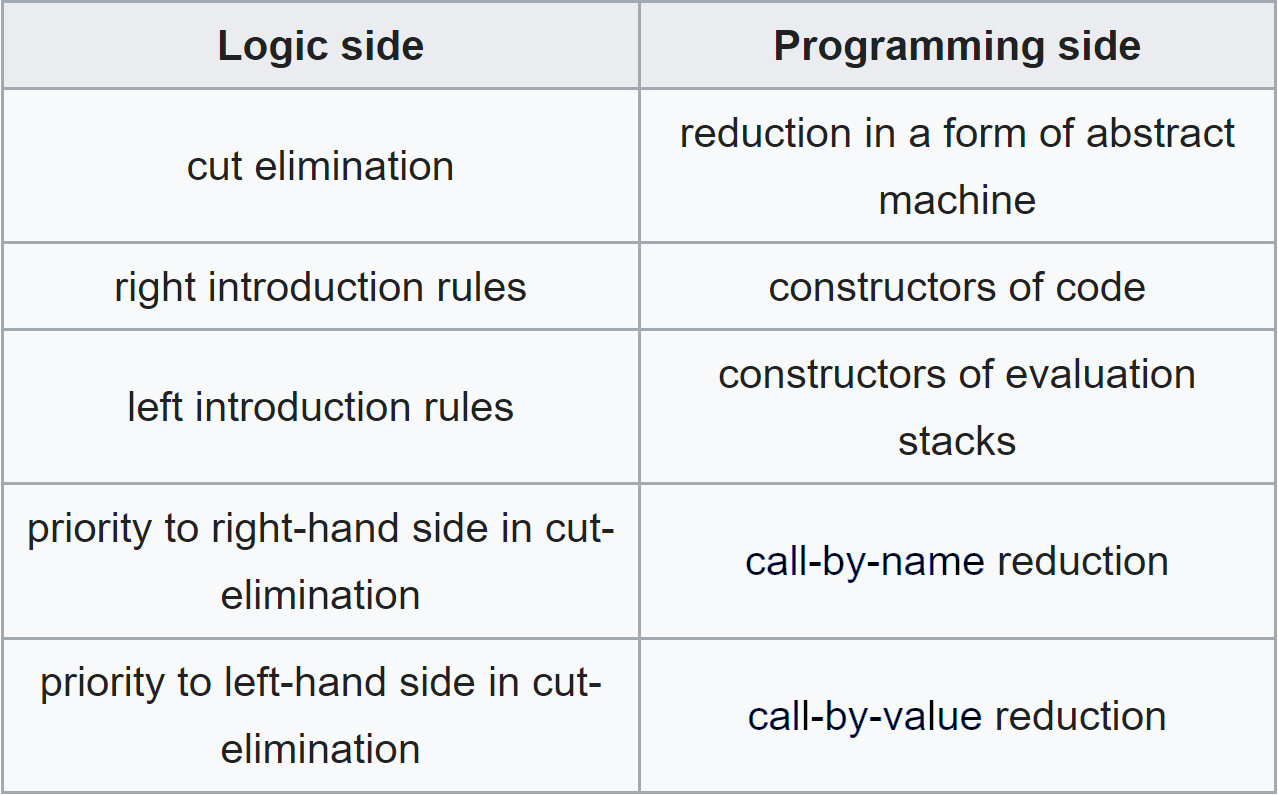
\includegraphics[width=\textwidth]{proofs_as_programs.png}
					\end{center}
					\vfill
				\end{subfigure}
			\end{figure}
	\end{frame}
	
	\begin{frame}{Motivation}		
		\begin{figure}[!tbp]
			\begin{subfigure}[t]{0.48\textwidth}
				\noindent We have a {\color{red}classical} prover...
				\begin{center}
					
\includegraphics[width=0.8\textwidth]{Vampire.png}
					\includegraphics[width=\textwidth]{CASC.png}
					\caption{CASC-28 Results}
				\end{center}
				\vfill
			\end{subfigure}
			\begin{subfigure}[t]{0.48\textwidth}
				\hfill...and {\color{red}intuitionistic} proofs are programs.
				\begin{center}
					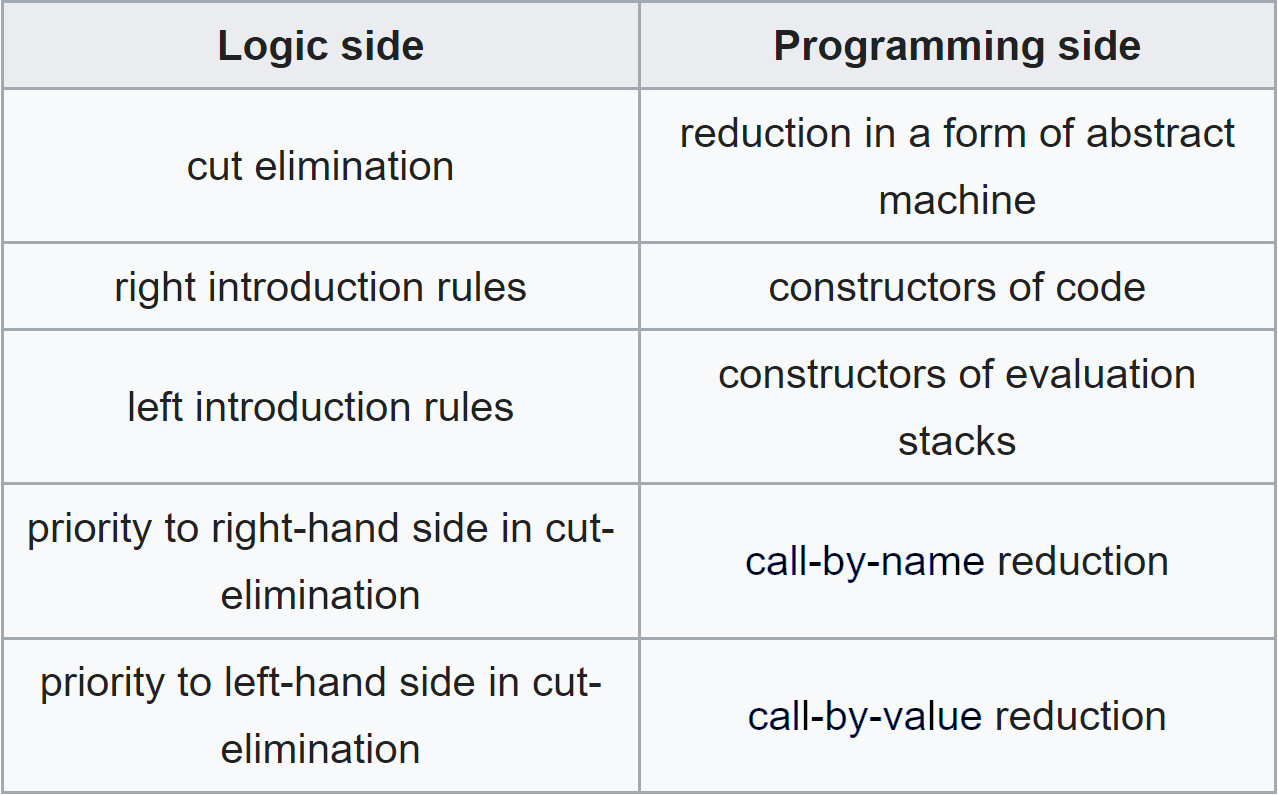
\includegraphics[width=\textwidth]{proofs_as_programs.png}
				\end{center}
				\vfill
			\end{subfigure}
		\end{figure}
	\end{frame}

	\begin{frame}{Kripke Semantics}
		\begin{figure}
			\centering
			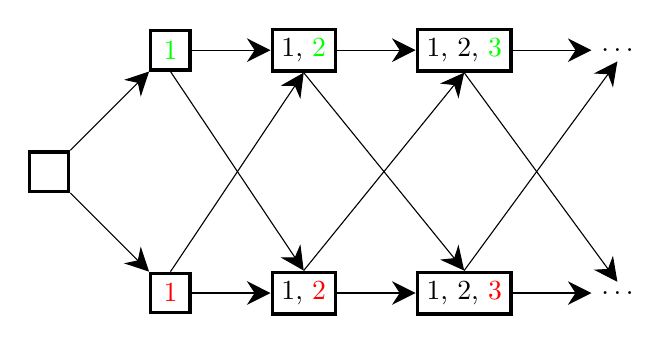
\begin{tikzpicture}[squarednode/.style={rectangle, draw, very thick, minimum size=5mm}]
				\node[squarednode]      (0)   [] {$ $};
				\node[squarednode]      (1r)   [above right=of 0] {{\color{green}$1$}};
				\node[squarednode]      (1l)   [below right=of 0] {{\color{red}$1$}};
				\node[squarednode]      (2r)   [right=of 1r] {{1, \color{green}$2$}};
				\node[squarednode]      (2l)   [right=of 1l] {{1, \color{red}$2$}};
				\node[squarednode]      (3r)   [right=of 2r] {{1, 2, \color{green}$3$}};
				\node[squarednode]      (3l)   [right=of 2l] {{1, 2, \color{red}$3$}};
				\node      (4r)   [right=of 3r] {{$\hdots$}};
				\node      (4l)   [right=of 3l] {{$\hdots$}};
				\draw[-{Stealth[length=3mm, width=3mm]}, color=black] (0.north east) -- (1r.south west);
				\draw[-{Stealth[length=3mm, width=3mm]}, color=black] (0.south east) -- (1l.north west);
				\draw[-{Stealth[length=3mm, width=3mm]}, color=black] (1r.east) -- (2r.west);
				\draw[-{Stealth[length=3mm, width=3mm]}, color=black] (1l.east) -- (2l.west);
				\draw[-{Stealth[length=3mm, width=3mm]}, color=black] (1l.north) -- (2r.south);
				\draw[-{Stealth[length=3mm, width=3mm]}, color=black] (1r.south) -- (2l.north);
				\draw[-{Stealth[length=3mm, width=3mm]}, color=black] (2r.east) -- (3r.west);
				\draw[-{Stealth[length=3mm, width=3mm]}, color=black] (2l.east) -- (3l.west);
				\draw[-{Stealth[length=3mm, width=3mm]}, color=black] (2l.north) -- (3r.south);
				\draw[-{Stealth[length=3mm, width=3mm]}, color=black] (2r.south) -- (3l.north);
				\draw[-{Stealth[length=3mm, width=3mm]}, color=black] (3r.east) -- (4r.west);
				\draw[-{Stealth[length=3mm, width=3mm]}, color=black] (3l.east) -- (4l.west);
				\draw[-{Stealth[length=3mm, width=3mm]}, color=black] (3l.north) -- (4r.south);
				\draw[-{Stealth[length=3mm, width=3mm]}, color=black] (3r.south) -- (4l.north);
			\end{tikzpicture}
			\vfill
			\caption{Kripke counter-model to $\neg(\neg \forall xA(x)\vee\neg \forall xB(x))$.}
		\end{figure}
	\end{frame}
	
	\begin{frame}{Encoding Kripke Semantics - Propositional Case}
		\begin{theorem}
			\label{thm:reduction-propositional}
			Let $\mathcal S$ be a set of flat and implicational clauses, $\mathcal F_\to\subseteq\mathcal S$ denote the subset implicational ones and $\Lambda$ denote the set of sequences without repetition over $\mathcal F_\to$. For each atom $A$ and $k\in\Lambda$ consider a new atom $A^k$. Obtain $\mathcal S^\#$ by including:
			\begin{itemize}
				\item $A^k\to A^{k\psi}$ for each atom $A$ occurring in $\mathcal S$, $k\in\Lambda$ and $\psi\in\mathcal F_\to$ not occurring in $k$.
				\item $A^k\to (B^k\circ C^k)$ for each $\circ\in\{\wedge,\vee\}$, $A\to (B\circ C)\in\mathcal S$, $k\in\Lambda$.
				\item $(A^k\circ B^k)\to C^k$ for each $\circ\in\{\wedge,\vee\}$, $A\to (B\circ C)\in\mathcal S$, $k\in\Lambda$.
				\item $(A^{k\psi}\to B^{k\psi})\to C^k$ for $\psi = (A\to B)\to C\in\mathcal S$, $k\in\Lambda$ if $\psi$ does not occur in $k$.
			\end{itemize}
			Then, $\bigwedge S\to P$ is intuitionistically valid iff $\bigwedge S^\#\to P^\epsilon$ is classically valid, where $\epsilon$ denotes the empty sequence.
		\end{theorem}
	\end{frame}
	
	\begin{frame}{Reducing the Encoding - Predicate Case}
		\begin{itemize}
			\item Essentially the same, but...
		\end{itemize}
	\end{frame}

	
	\begin{frame}{Implementation}
		\centering
		\begin{figure}
			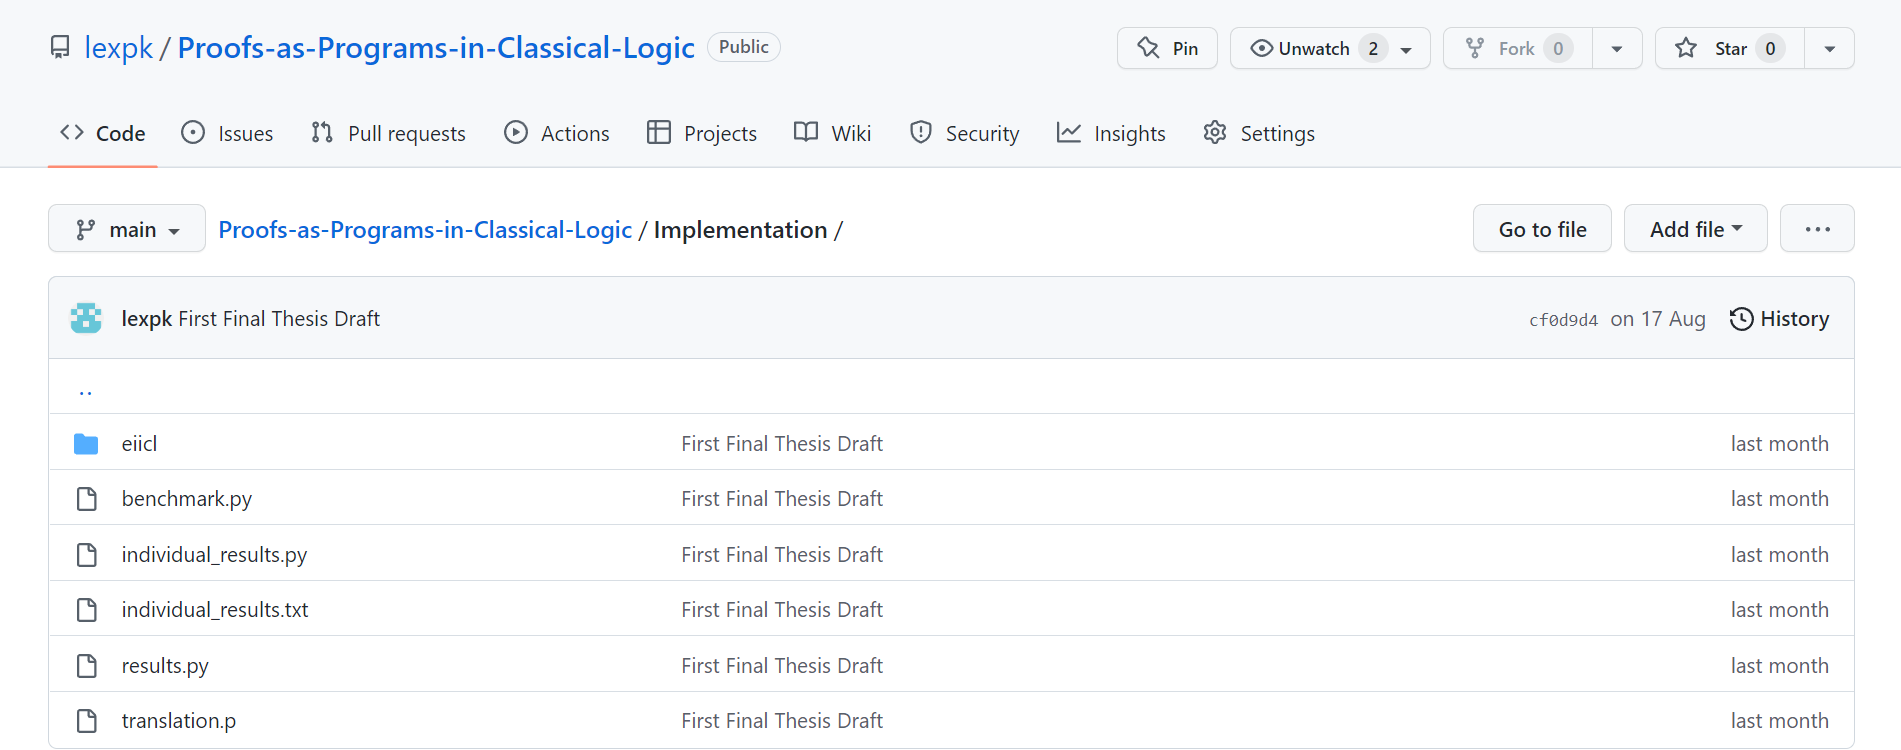
\includegraphics[width=\textwidth]{implementation.png}
		\end{figure}
		$\sim$3000 lines of rust code for the translation + $\sim$400 lines of python benchmarking
	\end{frame}


	\begin{frame}{Benchmark}
		
		\begin{figure}
			\begin{subfigure}[8]{0.4\textwidth}
				\def\firstcircle{(90:.75) circle (1.5)}
				\def\secondcircle{(210:.75) circle (1.5)}
				\def\thirdcircle{(330:.75) circle (1.5)}
				\begin{tikzpicture}
					\begin{scope}[shift={(3cm,-5cm)}, opacity=0.5, blend mode=multiply]
						\fill[red] \firstcircle;
						\fill[green] \secondcircle;
						\fill[blue] \thirdcircle;
						\draw node {$491$};
						\draw node at (30:1.2) {$30$};
						\draw node at (150:1.2) {$42$};
						\draw node at (270:1.2) {$22$};
						\draw node at (90:1.8) {$8$};
						\draw node at (210:1.8) {$2$};
						\draw node at (330:1.8) {$417$};
					\end{scope}
				\end{tikzpicture}
			\end{subfigure}
			\begin{subfigure}[8]{0.4\textwidth}
				\vspace*{-.5cm}
				\begin{tabular}{l|c|c}
					Embedding&571&21.4\%\\
					Embedding (idem.)&557&20.9\%\\
					ileanCoP 1.2&875&32.8\%\\
					nanoCoP-i 2.0&858&32.1\%\\\hline
					Total&2669&100\%
				\end{tabular}
			\end{subfigure}
			\vfill
			\caption{Number of theorems proven via our Embedding (red) with extra axioms (green) and a combination of existing state-of-the-art provers (blue) on the ILTP benchmark set.}
		\end{figure}
	\end{frame}
	
\begin{frame}[standout]
	\Huge\textsc{Thank You}
\end{frame}
	
\end{document}